% !TEX root = ../thesis.tex
Beryllium metal is ablated with an Nd:YAG laser and trapped in a linear Paul trap. Laser cooling is applied with a 313nm laser. Pure O$_2$ gas is introduced into the chamber via leak valve to react with the ions. Remaining reactants and charged reaction products are ejected into a time-of-flight mass spectrometer (TOF) where the various masses of ions can be determined.


With the introduction of \ce{O2} into the chamber, we consider all the possible reaction products of \ce{Be+ + O2}

\begin{align}
	\ce{Be+(^2S1/2) + O2 & -> no reaction} \label{r: Be(S)+O2->O2+} \\
	\ce{& -> no reaction} \label{r: Be(S)+O2->BeO+} \\
	\ce{Be+(^2P3/2) + O2 & -> O2+ + Be} \label{r: Be(P)+O2->O2+} \\
	\ce{& -> BeO+ + O2} \label{r: Be(P)+O2->BeO+}
\end{align}

Without excitation into the \ce{^2P3/2} manifold, reactions \ref{r: Be(S)+O2->O2+} and \ref{r: Be(S)+O2->BeO+} are endothermic by 2.75 eV and 1.1 eV, respectively. Despite the fact that reaction \ref{r: Be(P)+O2->BeO+} is energetically allowed, it is never seen with laser cooling.

Without 313 nm light, the \ce{Be+} ions stay in the \ce{^2S1/2} ground state, but with a ion trap depth > 3 eV, there are portions of the ion cloud with enough energy to still proceed with the production of \ce{BeO+}. Without the laser cooling, we observe the disappearance of \ce{BeO+} from the trap due to exciting the molecule into a pre-dissociative state.\todo{cite beo}

\begin{figure}[H]
	\centering
	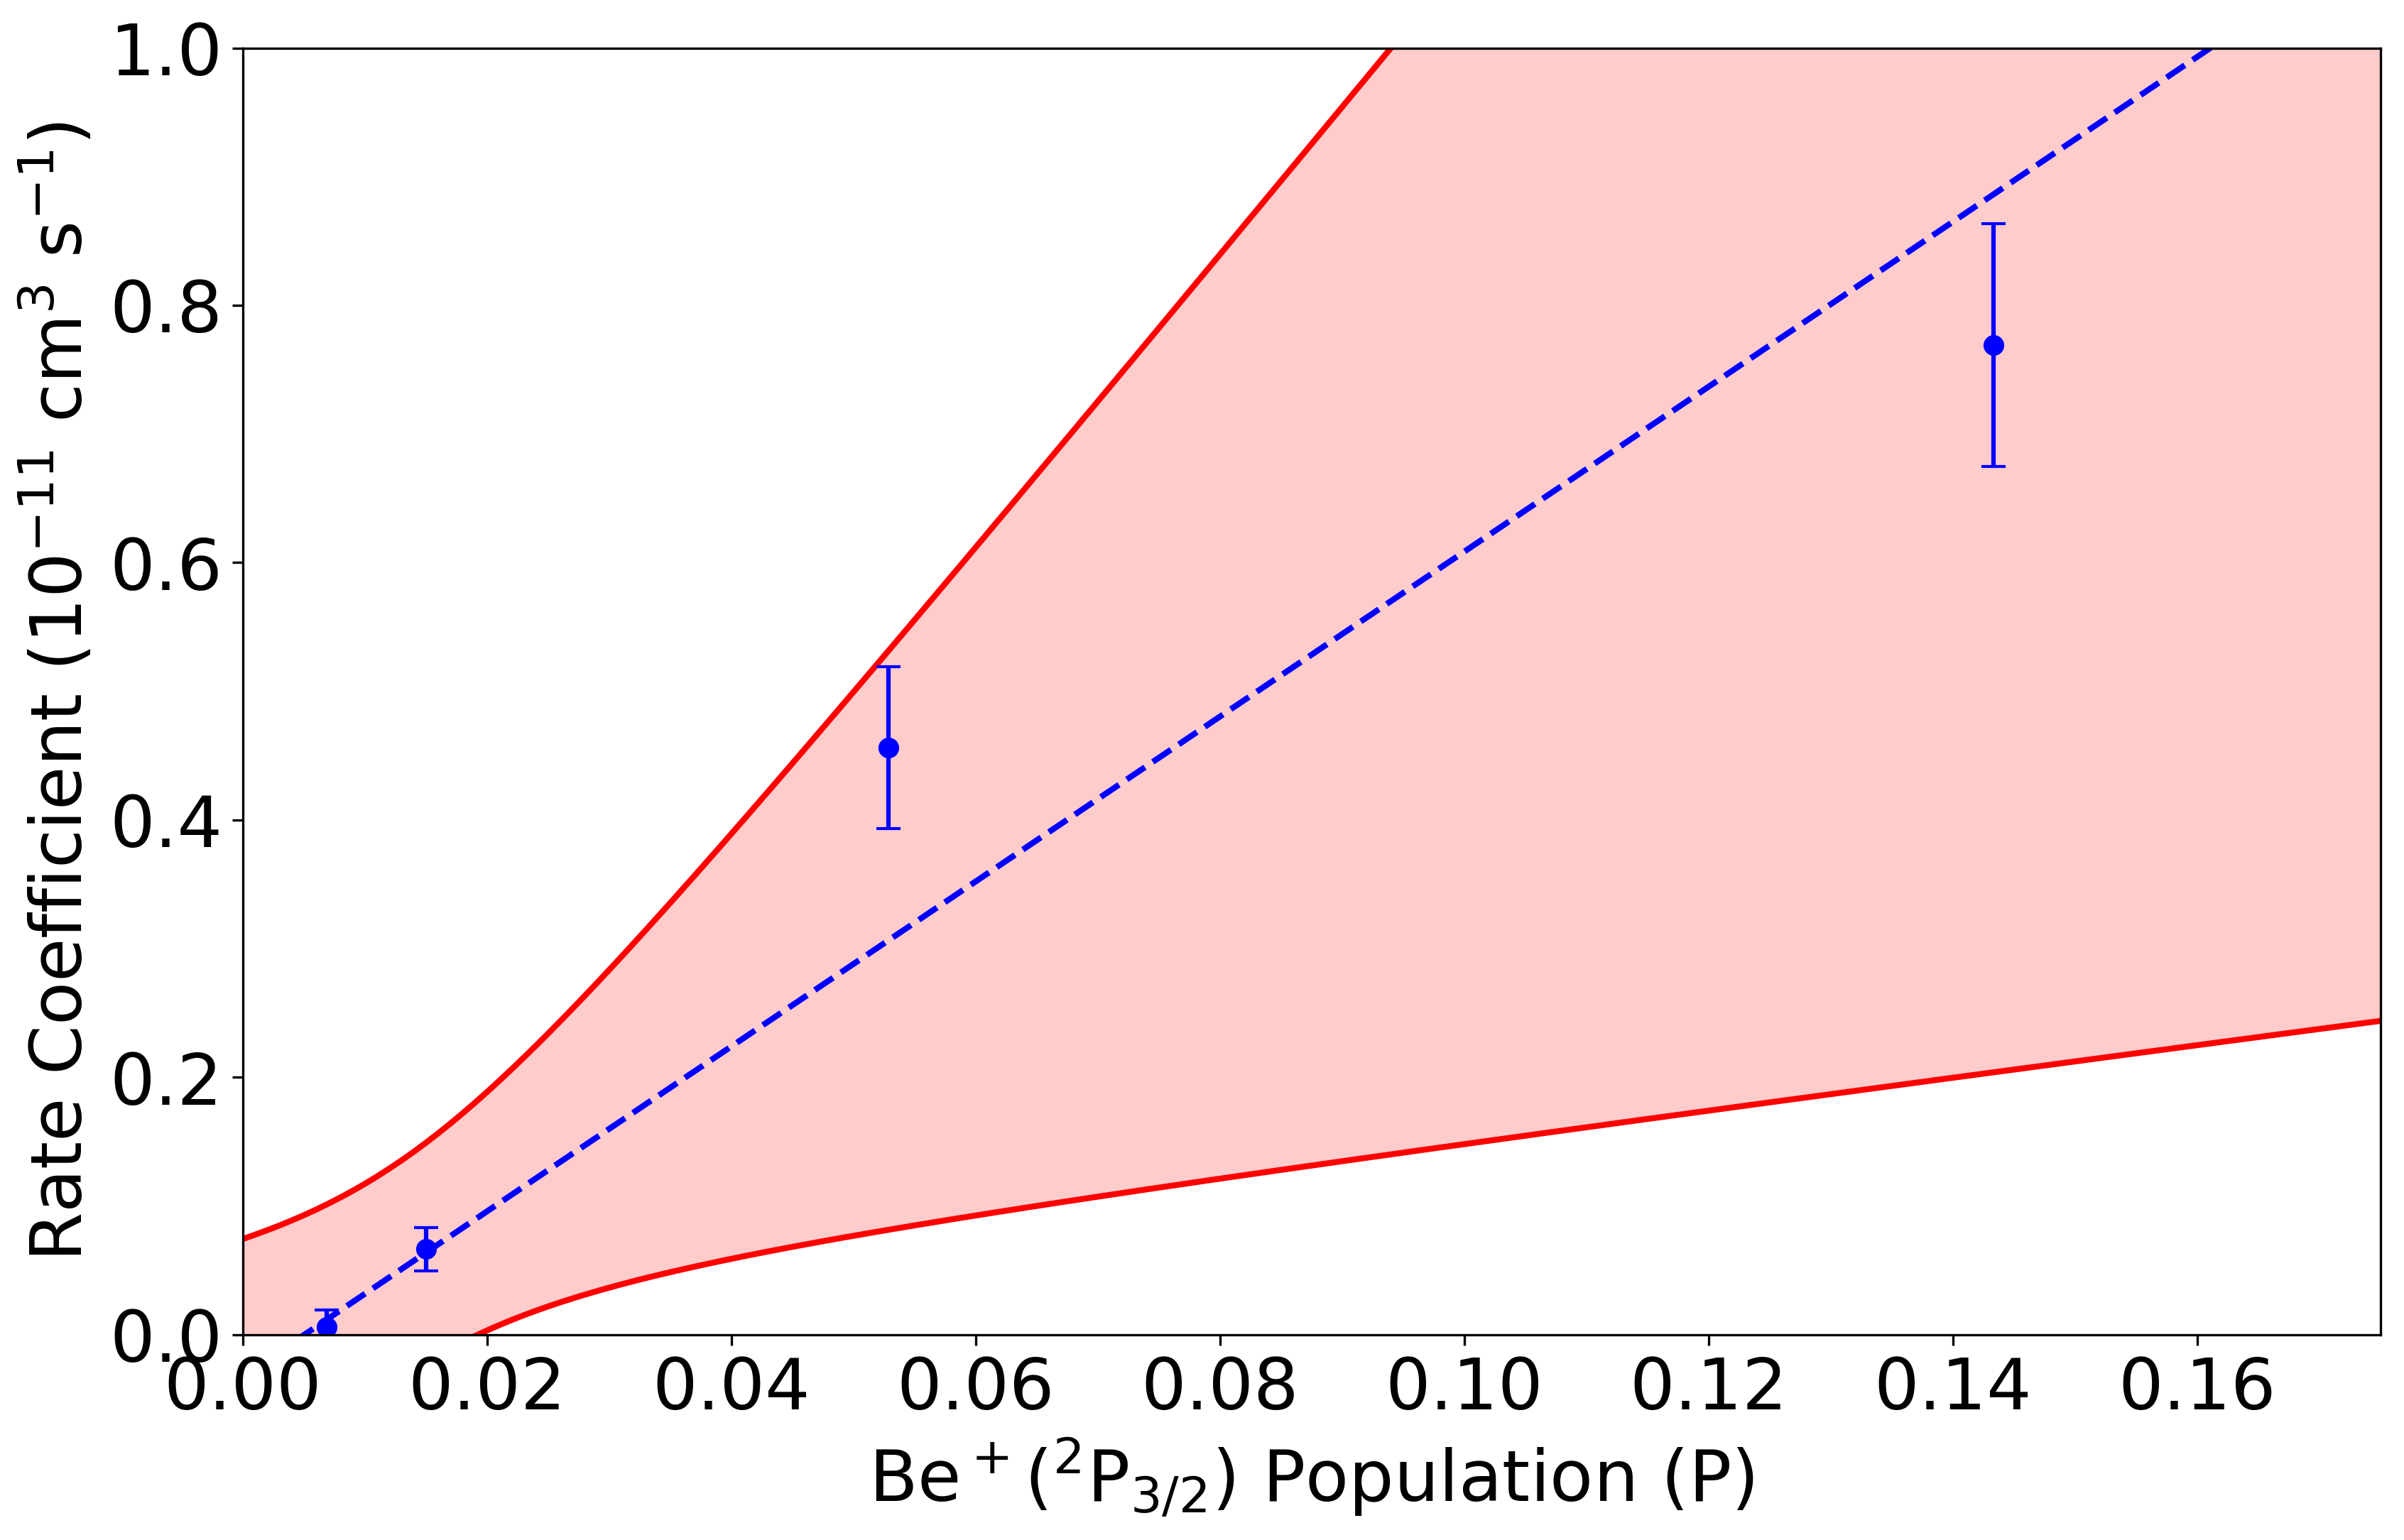
\includegraphics[width=0.7\textwidth]{images/Be_O2_P_state.png}
	\caption{\label{fig: p-state} A linear dependence on the rate constant for reaction \ref{r: Be(P)+O2->O2+} as a function of P state excitation. $k = (6 \pm 1) \times 10^{-11} P + (-0.03 \pm 0.16) \times 10^{-11}$}
\end{figure}

% \begin{figure}[H]
%	 \centering
%	 \includegraphics[width=0.5\textwidth]{p_state_no_b.png}
%	 \caption{\label{fig: p-state} A linear dependence on the rate constant for reaction \ref{eq: o2+} as a function of P state excitation. Fit $(5.45 \pm 1.03) \times 10^{-11} P$}
% \end{figure}

\begin{figure}[H]
	\centering
	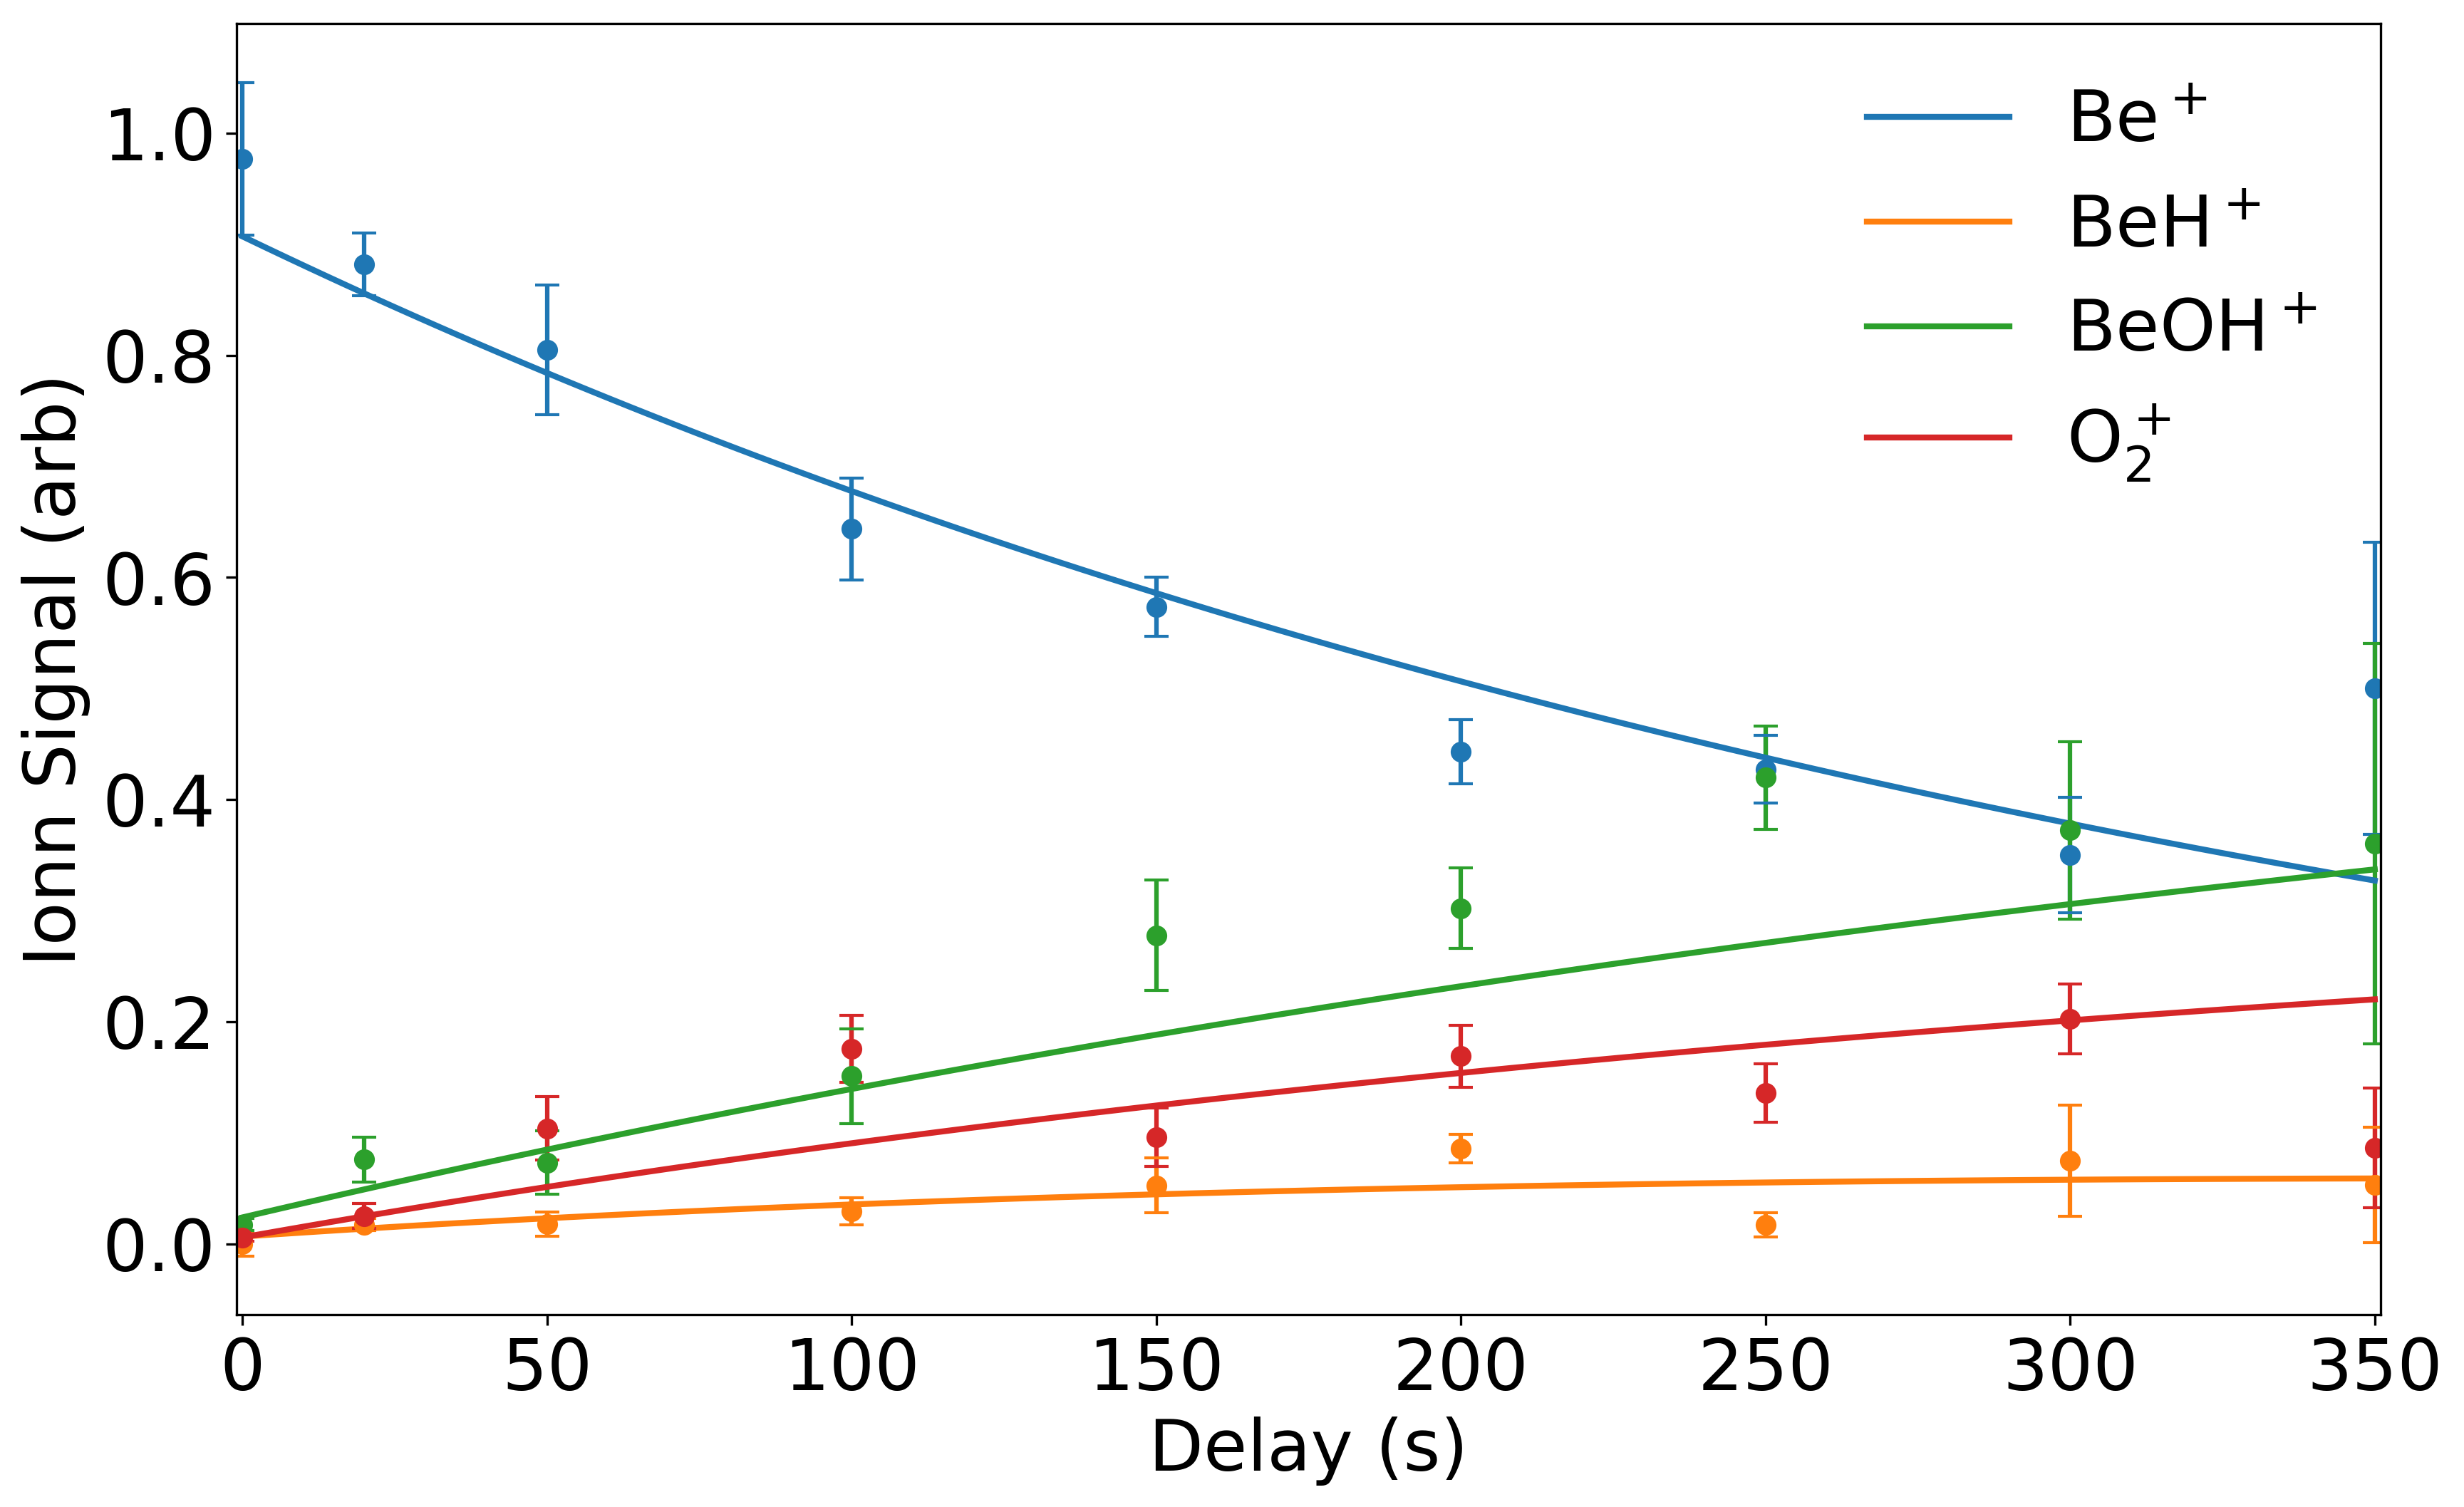
\includegraphics[width=0.7\textwidth]{images/Be_O2_laser_fit.png}
	\caption{\label{fig: laser fit} Shared fitting of trapped products with 14\% p-state excitation.}
\end{figure}

\begin{figure}[H]
	\centering
	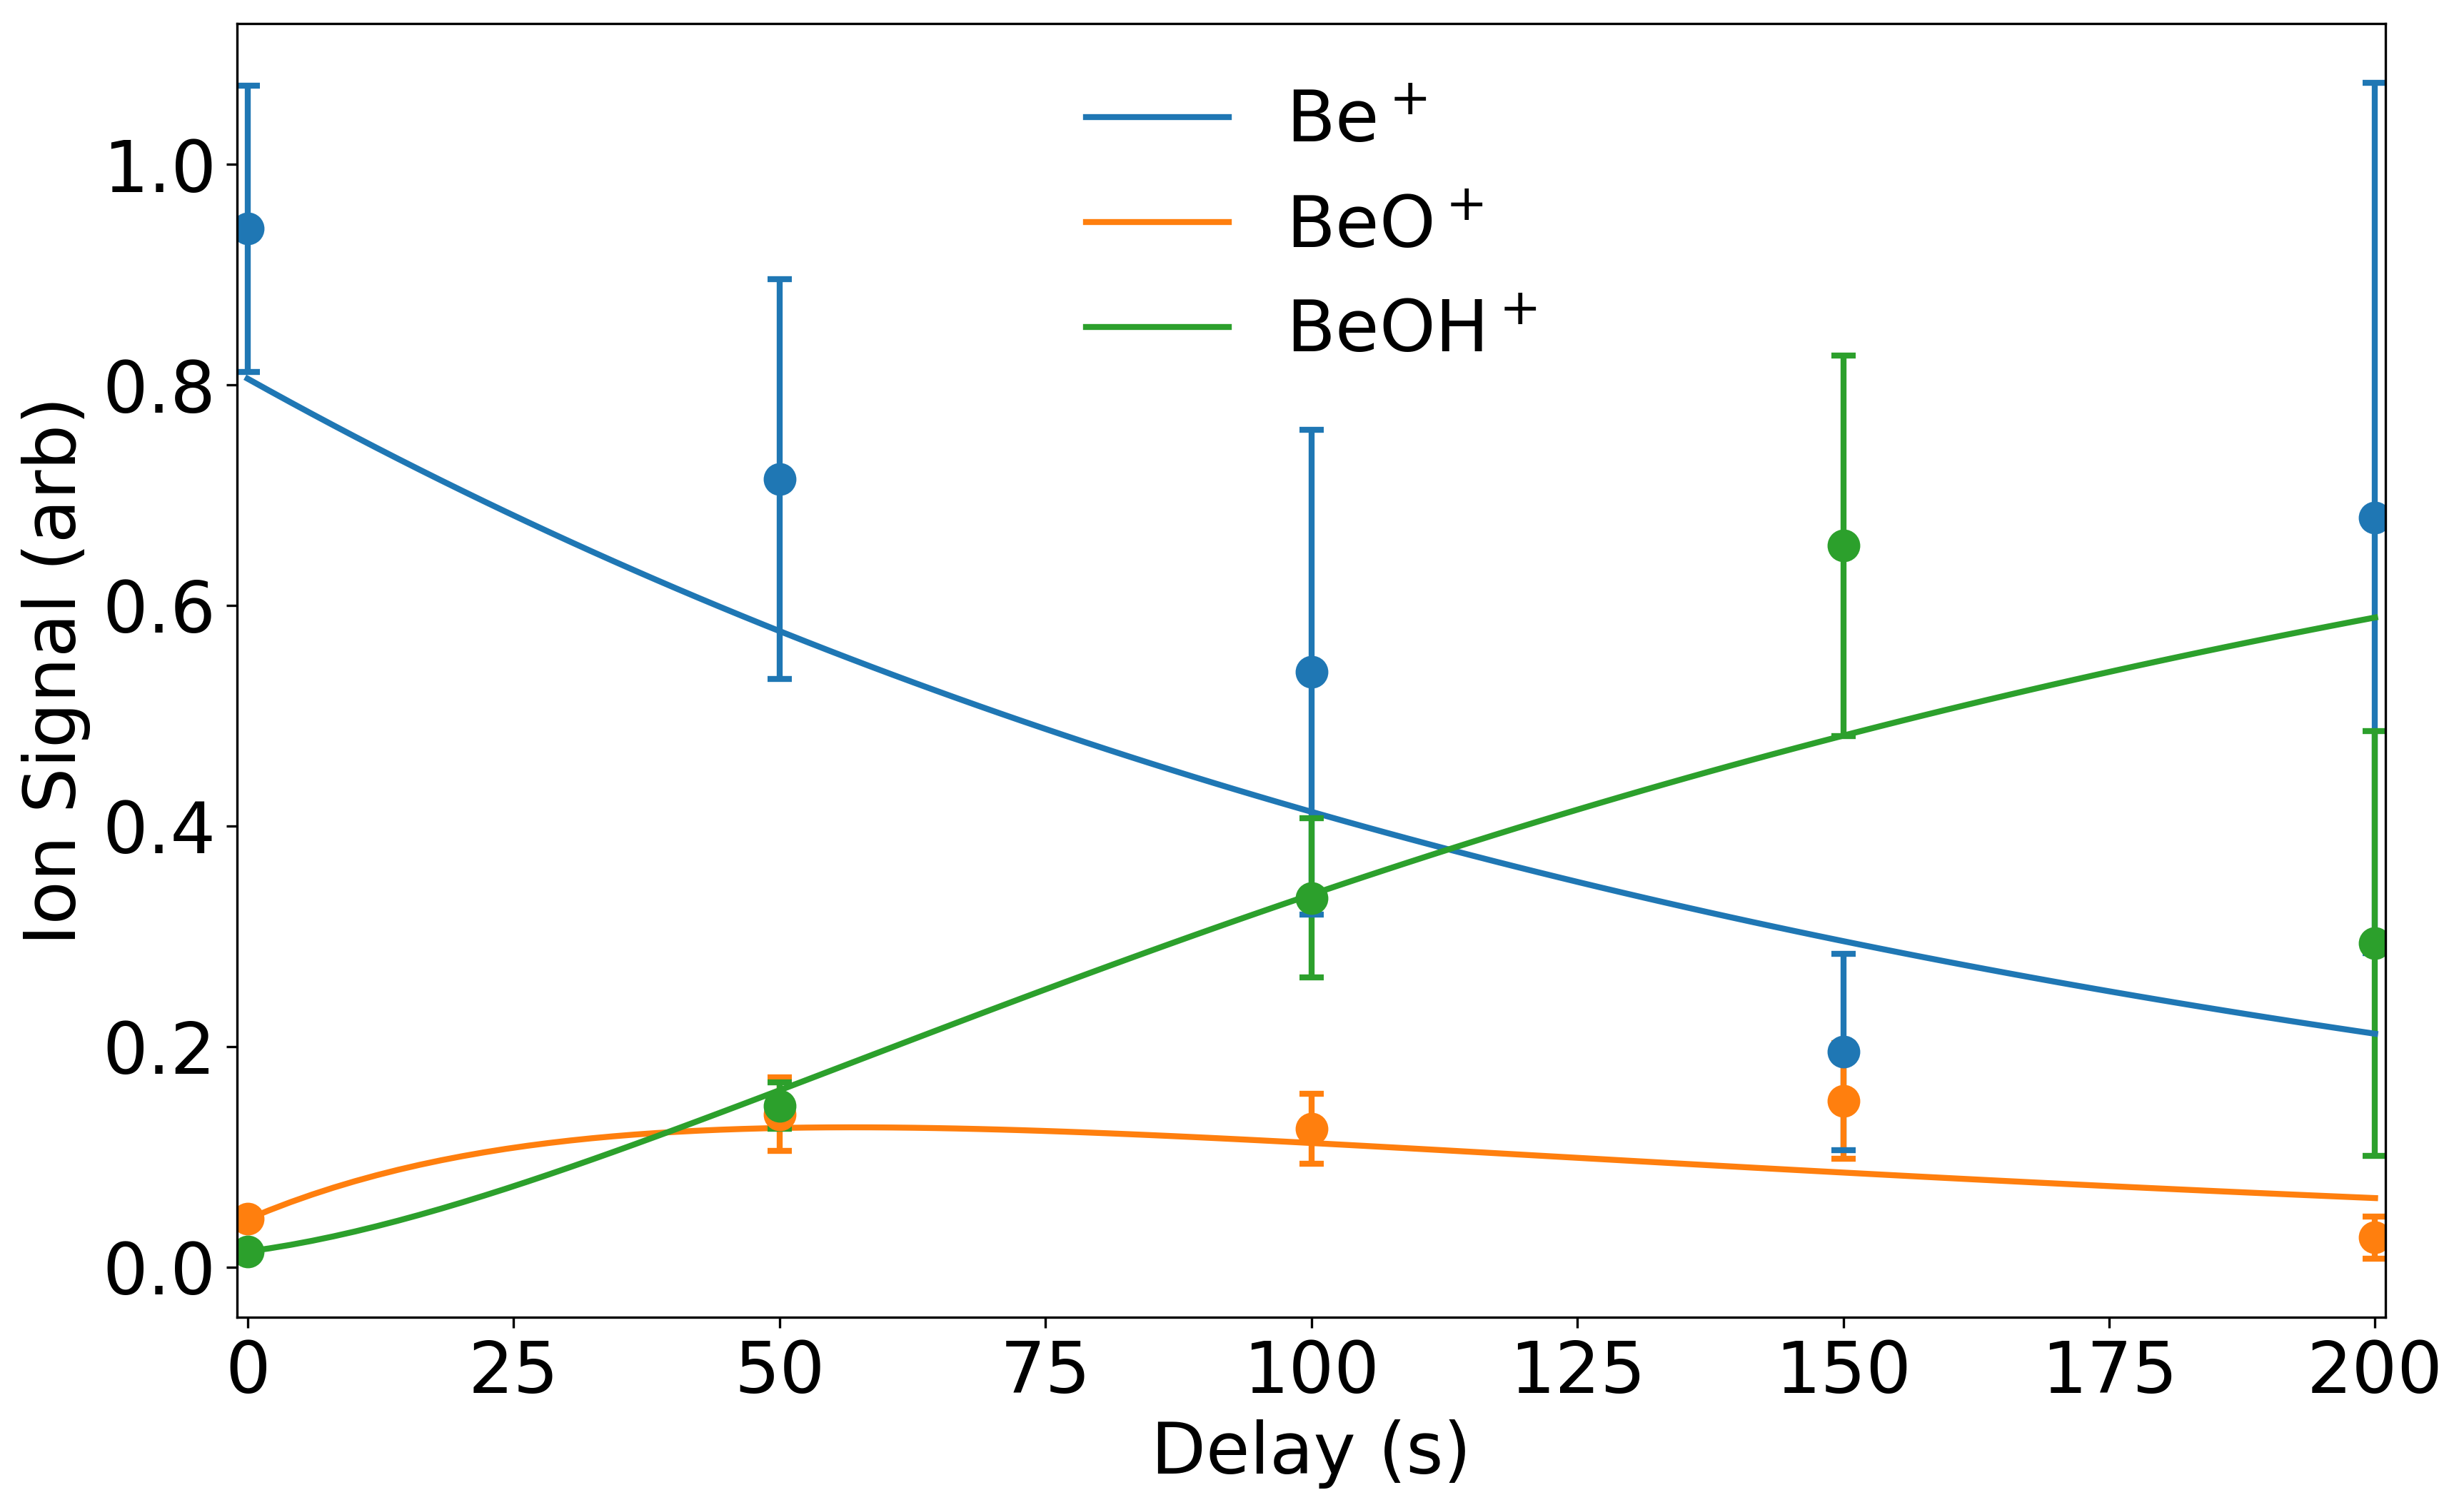
\includegraphics[width=0.7\textwidth]{images/Be_O2_no_laser_fit.png}
	\caption{\label{fig: no laser fit} Shared fitting of trapped products where \ce{Be+} was exposed to \ce{O2} without the 313 nm light.}
\end{figure}

\begin{figure}[H]
	\centering
	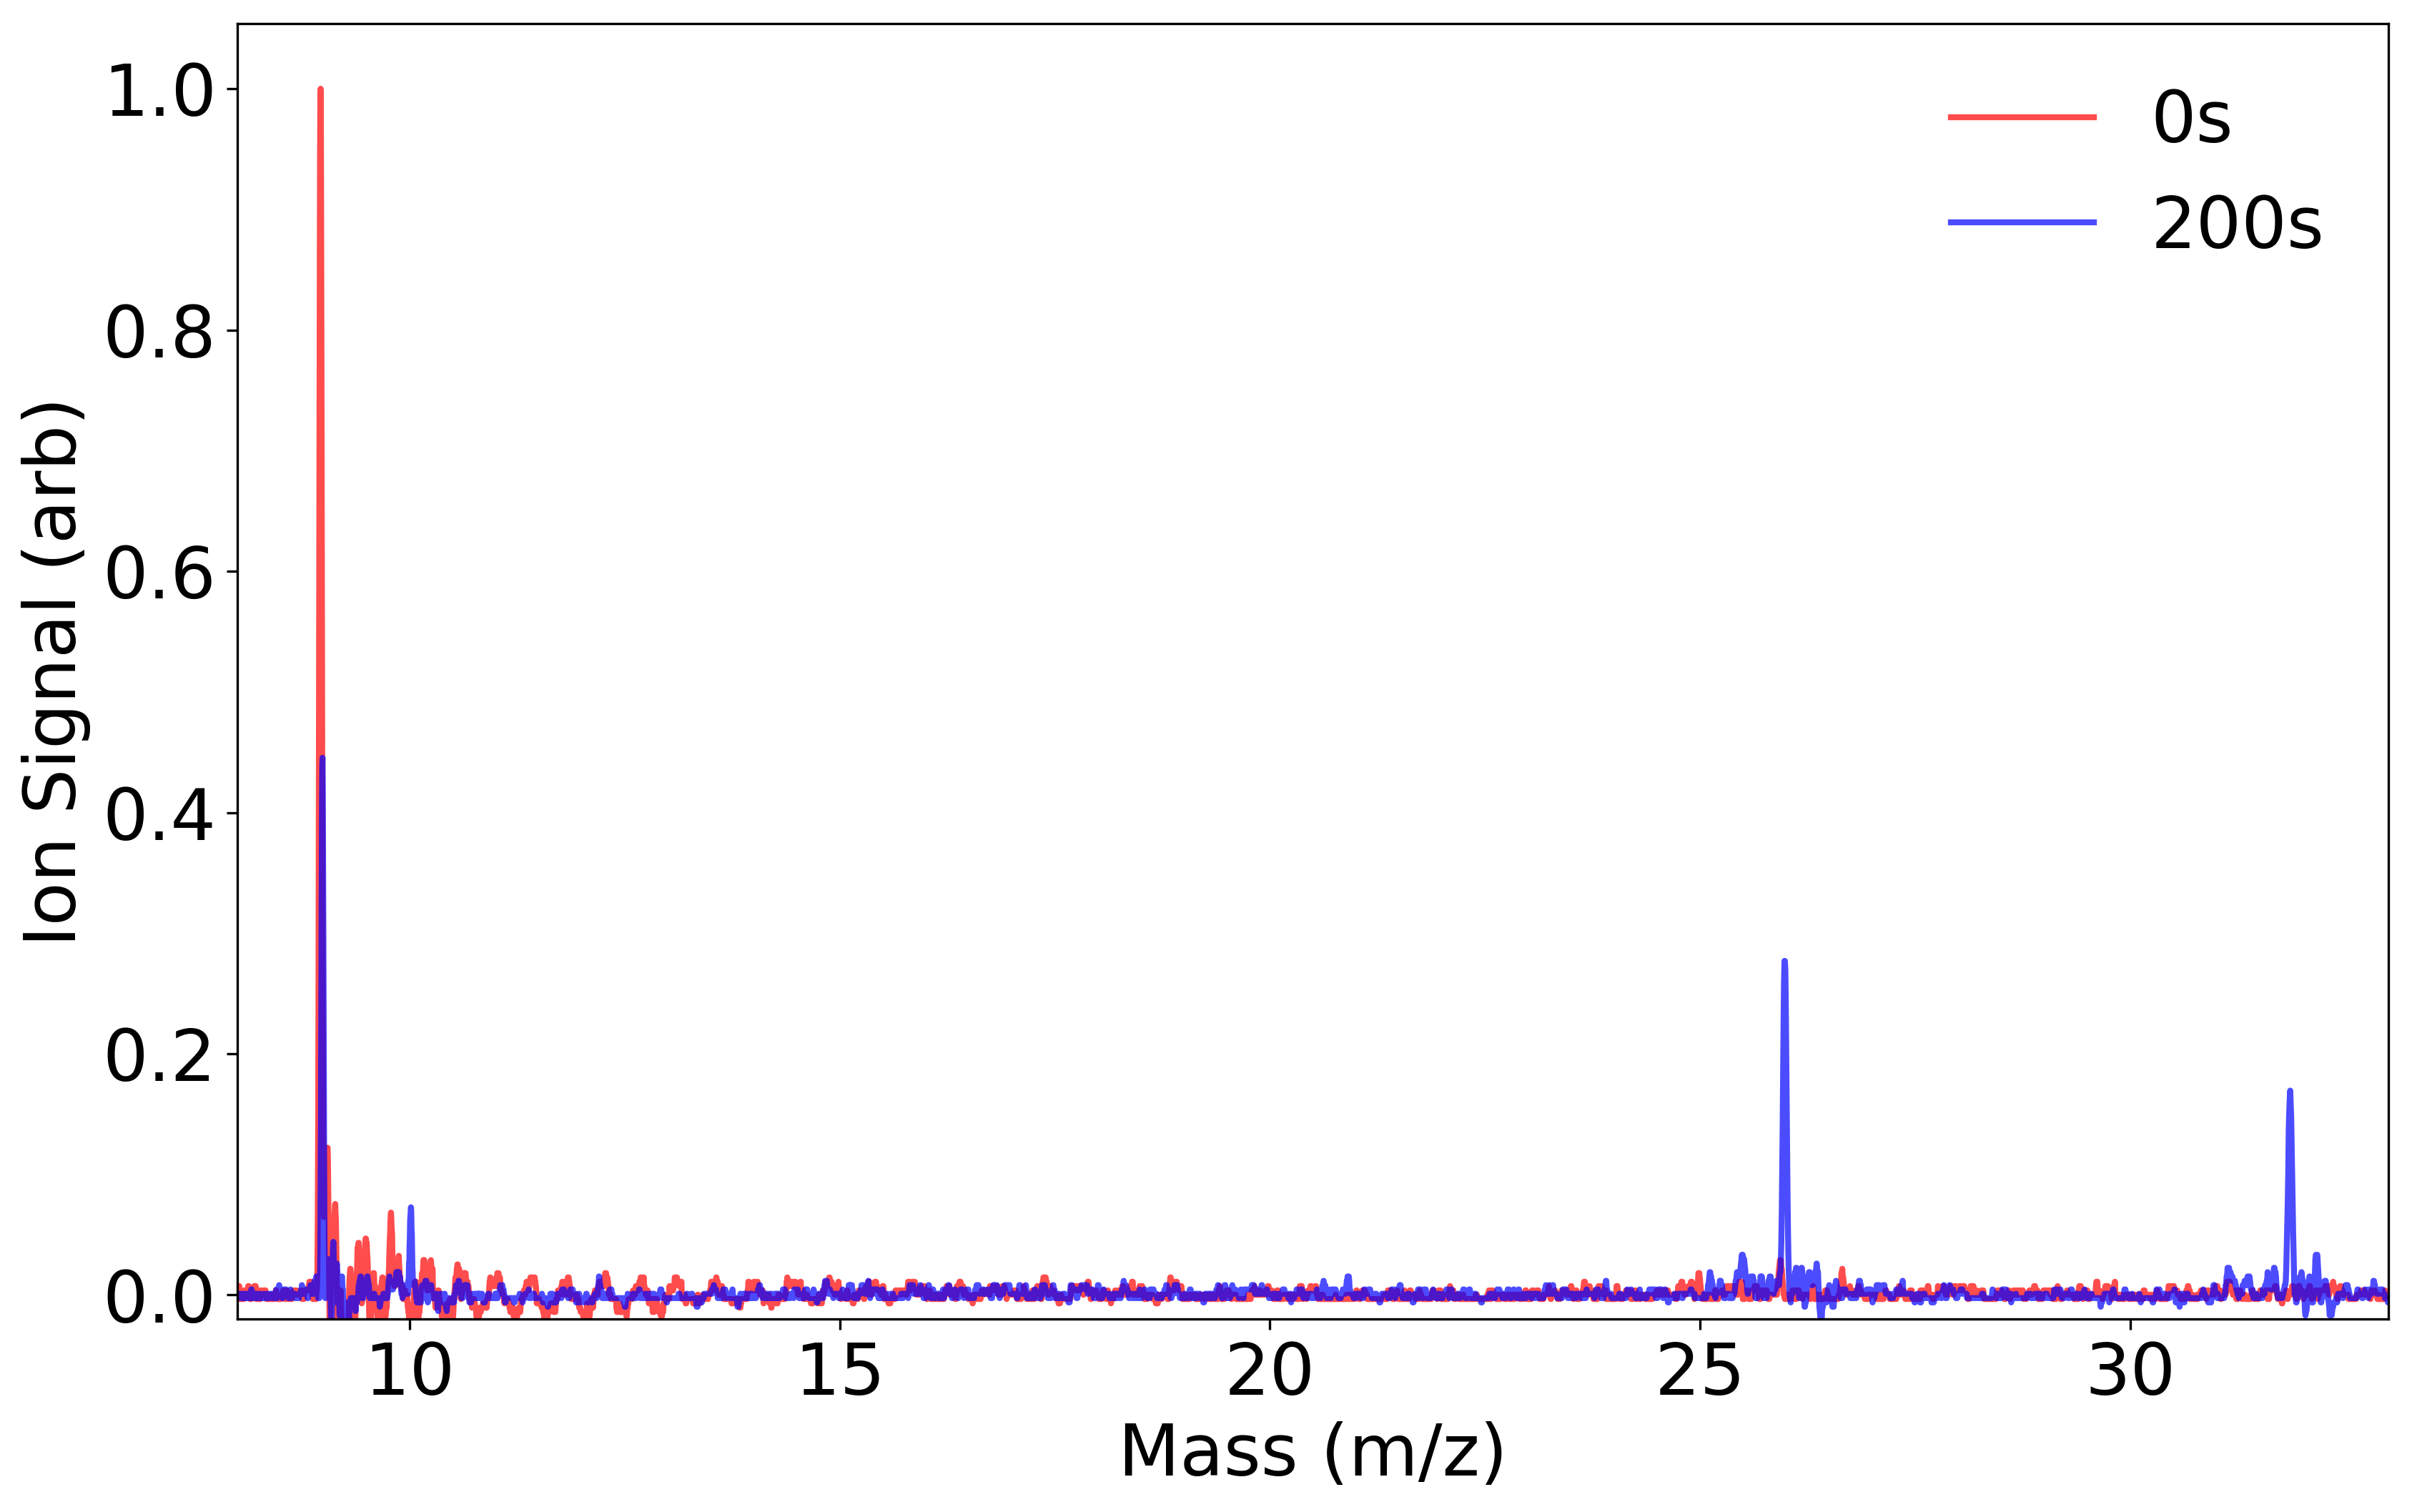
\includegraphics[width=0.7\textwidth]{images/Be_O2_laser_TOF.png}
	\caption{TOF traces for data taken with 14\% p-state excitation at 0s and 200s showing no products at 0s, distinct peaks for reaction products \ce{BeH+}, \ce{BeOH+}, and \ce{O2+}, but an absence of \ce{BeO+}.}
	\label{fig: laser TOF}
\end{figure}

\begin{figure}[H]
	\centering
	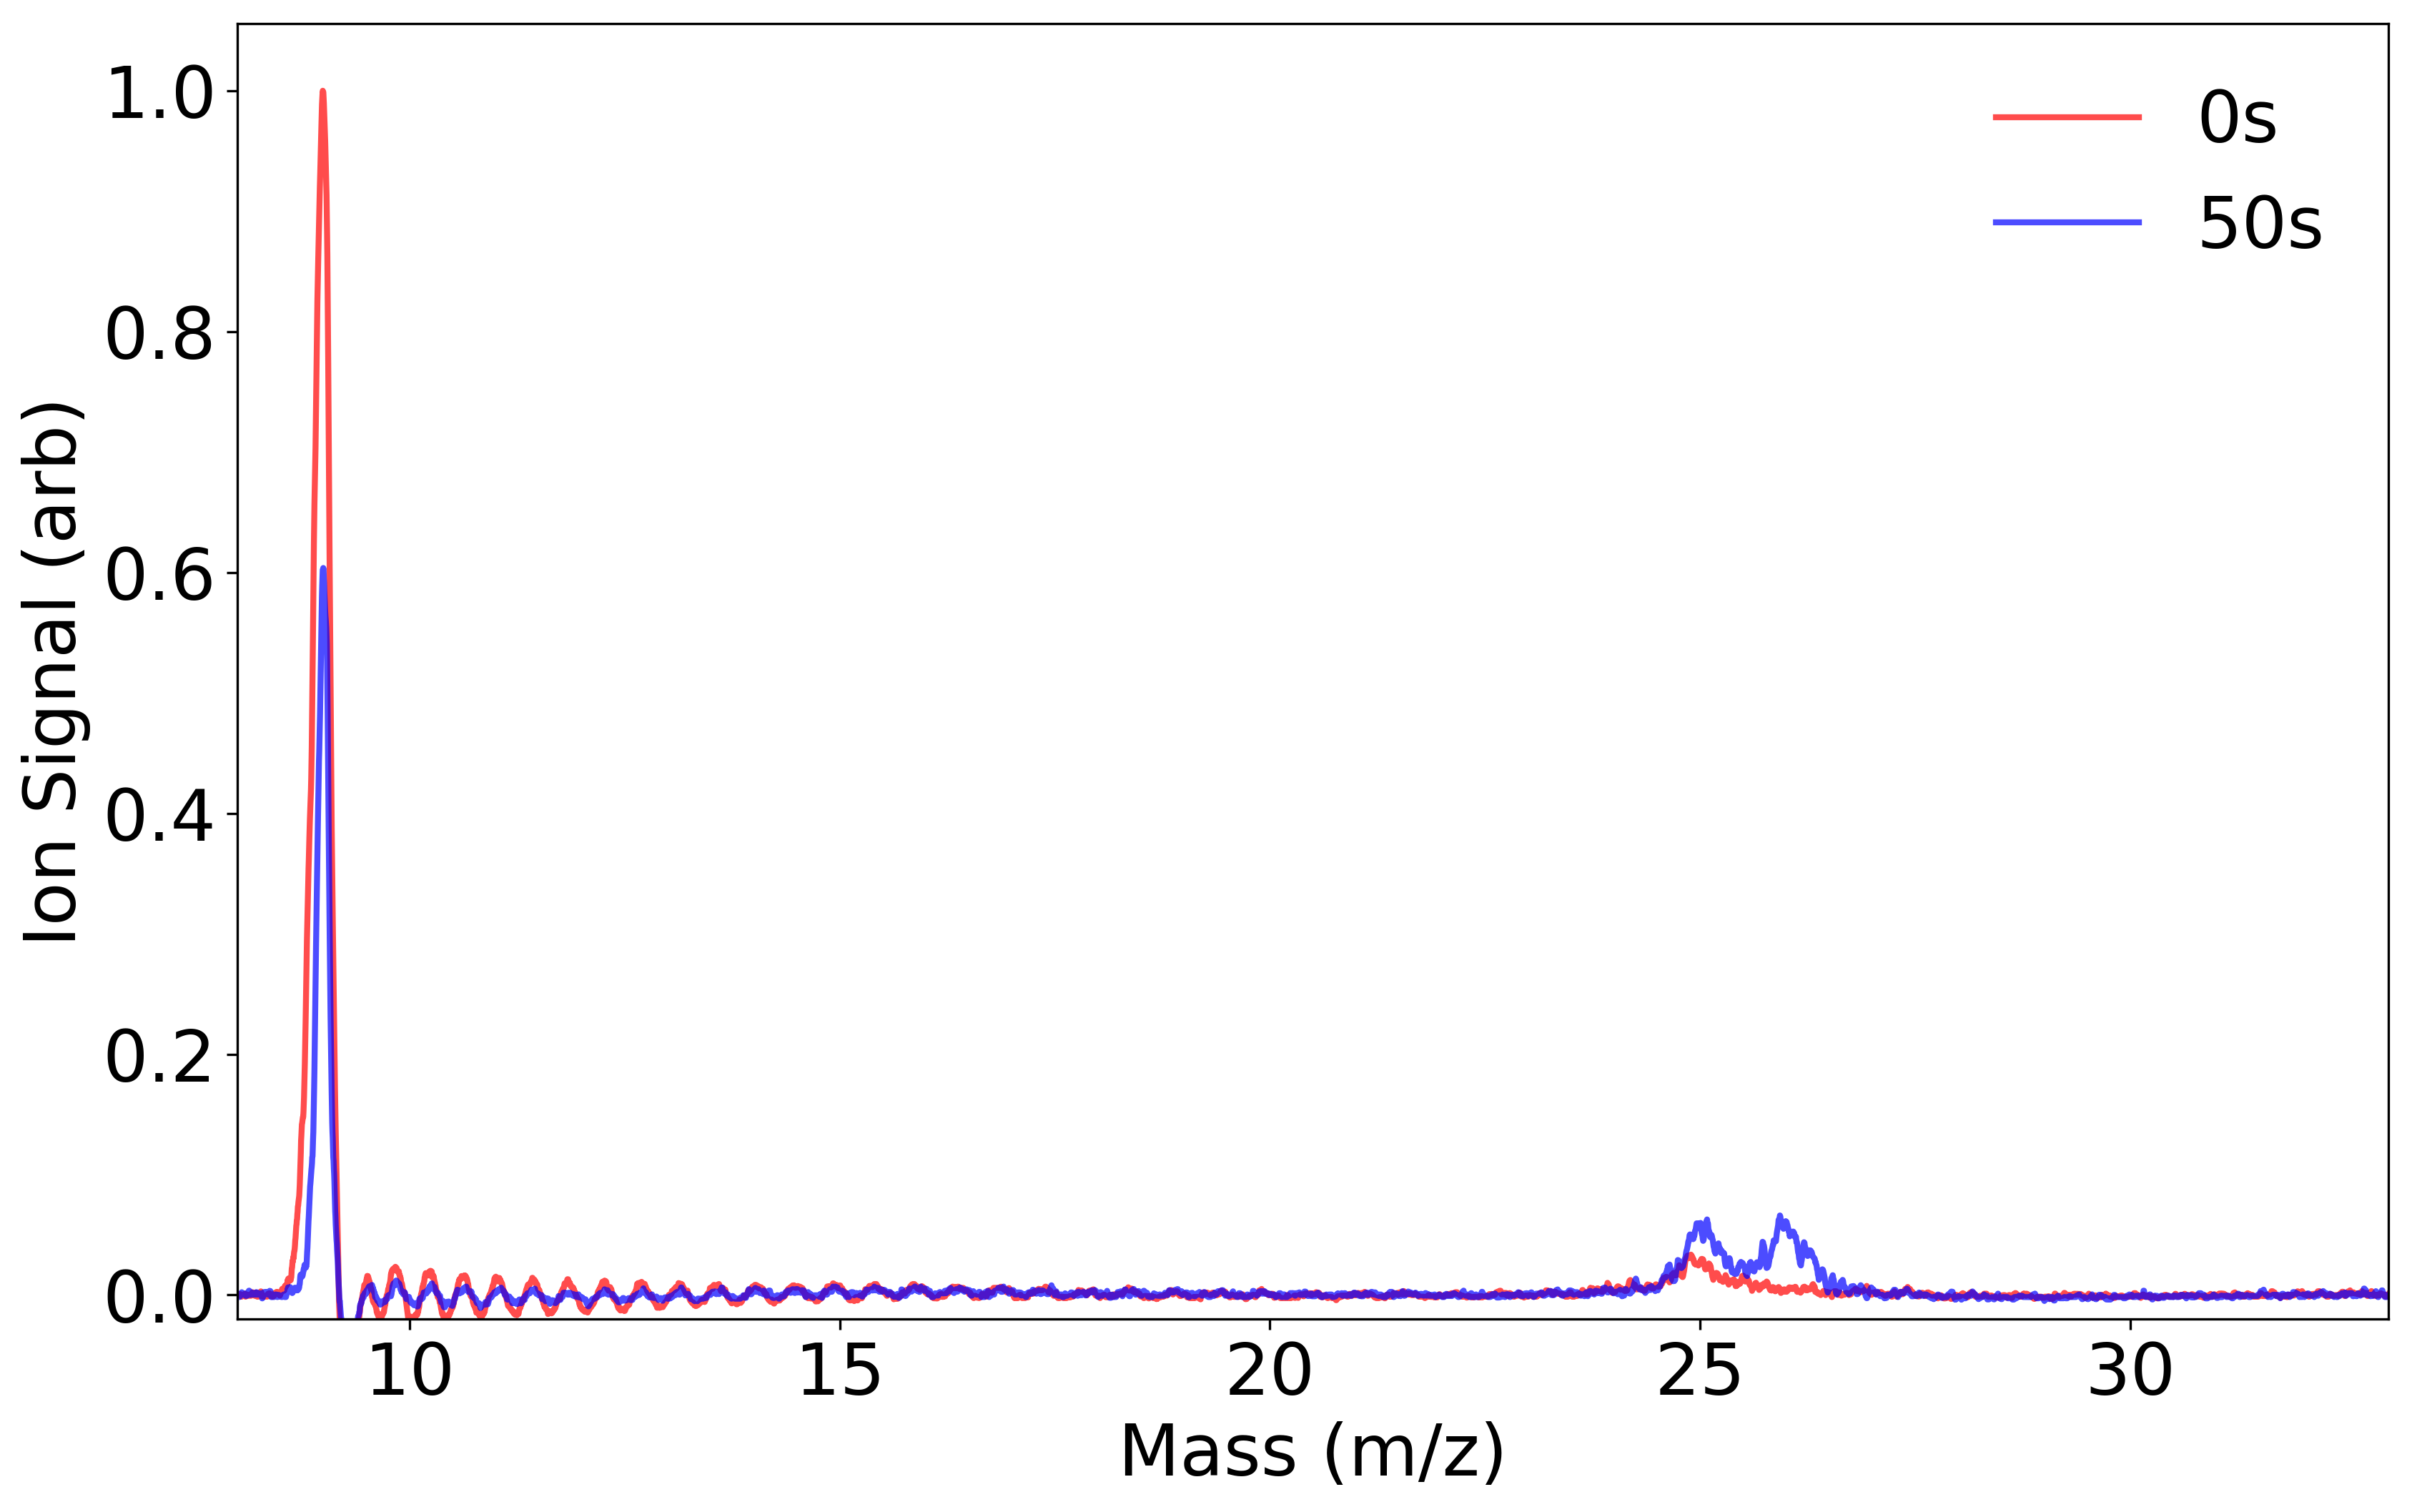
\includegraphics[width=0.7\textwidth]{images/Be_O2_no_laser_TOF.png}
	\caption{TOF traces for data taken with without laser excitation at 0 s and 50 s showing residual \ce{BeOH+} at 0 s, but only an inclusion of \ce{BeO+} at 50 s. More endothermic product channels of \ce{BeH+} and \ce{O2+} are absent.}
	\label{fig: non laser TOF}
\end{figure}

Considering state counting, reactions \ref{r:} and \ref{eq: o} have been measured to have branching ratios that vary from 60:40 (CO$^+$:O$^+$) to 30:70 in the other direction. By looking at experimental data as well as the theoretical state counting, we find the ratio to be pretty definitively 60:40.
